\section{Gaussian Channel with Ergodic $\vb{H}$}
%%%%%%%%%%%%%%%%%%%%%%%%%%%%%%%%%%%%%%%%%%%%%%%%%%%%%%%%%%%%%%%%%%%
%%%%%%%%%%%%%%%%%%%%%%%%%%%%%%%%%%%%%%%%%%%%%%%%%%%%%%%%%%%%%%%%%%%
\subsection{Introduction to the problem}
\begin{frame}{Introduction}

We now consider the case when the matrix $\vb{H}$ is i.i.d. random and ergodic. Ergodicity comes into play to ensure that the capacity is the actual bound as matrix is randomly changing over time.

\medskip
We assume that $\vb{H}$ is independent of both $\vb{x}$ and $\vb{n}$, and that the specific realization $H$ is know at the receiver (while the transmitter only knows its distribution). Thus, we can equivalently say that the channel yields the couple $(\vb{y,H})$.

\medskip
We will further assume that the entry of $\vb{H}$ are i.i.d. zero-mean Complex Gaussian, with independent real and imaginary parts, each with variance $\frac{1}{2}$.

\medskip
In other words we are considering a Rayleigh fading channel for each component and enough physical separation within transmitting and receiving antennas to achieve independence between the entries of $\vb{H}$.

\end{frame}

%%%%%%%%%%%%%%%%%%%%%%%%%%%%%%%%%%%%%%%%%%%%%%%%%%%%%%%%%%%%%%%%%%%
%%%%%%%%%%%%%%%%%%%%%%%%%%%%%%%%%%%%%%%%%%%%%%%%%%%%%%%%%%%%%%%%%%%
\subsection{Capacity-achieving Distribution}
\begin{frame}[allowframebreaks]{Capacity-achieving Distribution}
This time, we can compute the mutual information as follows
\begin{align*}
\begin{split}
I(\vb{x;(y,H)}) &= I(\vb{x;H}) + I(\vb{x;y|H})\\
&= I(\vb{x;y|H})\\
&= \Exp[\vb{H}]{I(\vb{x;y|H}=H)}
\end{split}
\end{align*}

We know that for a deterministic $H$, the maximizer $\vb{x}$ takes the form of a zero-mean \cscg{} with covariance $Q$, and $\Psi(Q,H) = \log\det(I_r + HQ\herm{H})$ is the corresponding maximal mutual information.

\medskip
We thus need to maximize
$$\Psi(Q) = \Exp{\Psi(Q,\vb{H})} = \Exp{\log\det(I_r + \vb{H}Q\herm{\vb{H}})}$$
over the choice of positive semi-definite $Q$, such that $\tr(Q)\leq P$.

%%%%%%%%%%%%%%%%%%%%%%%%%%%%%%%%%%%%%%%%%%%%%%%%%%%%%%%%%%%%%%%%%%%
\framebreak

Since $Q$ is positive semi-definite, we can write it as $Q = W\Delta\herm{W}$, where $W$ is unitary and $\Delta$ is non-negative diagonal. Thus
$$\Psi(Q) = \Exp{\log\det(I_r + (\vb{H}W)\Delta\herm{(\vb{H}W)})}$$
It can be shown that $\vb{H}W$ has the same distribution as $\vb{H}$ (since $W$ is unitary and $\vb{H}$ has i.i.d. entries), and thus $\Psi(Q)=\Psi(\Delta)$. It follows that we can focus on positive semi-definite diagonal $Q$.

\medskip
Consider the permutation matrix $\Pi$ (which is orthogonal, thus unitary) and define $Q^\Pi \triangleq \Pi Q \Pi^T$. Again, we note that $\Psi(Q^\Pi) = \Psi(Q)$. Also, note that if $Q$ is diagonal, also $Q^\Pi$ is diagonal and they share the same determinant (the main diagonal is only shuffled).

%%%%%%%%%%%%%%%%%%%%%%%%%%%%%%%%%%%%%%%%%%%%%%%%%%%%%%%%%%%%%%%%%%%
\framebreak

Note that the transformation $Q\rightarrow I_r+HQ\herm{H}$ is linear and preserves positive definiteness, and know that the $\log\det$ function is concave over the closed cone of positive semi-definite matrices.\\
Thus $Q\rightarrow \Psi(Q)$ is concave.

\medskip
Let's define
$$\tilde{Q} = \frac{1}{t!}\sum_\Pi Q^\Pi$$
Note that $\tilde{Q}=\alpha I_t$ for some $\alpha$ for any $Q$, that $\tr(\tilde{Q})=\tr(Q)$ and $\Psi(\tilde{Q})\geq\Psi(Q)$.

%%%%%%%%%%%%%%%%%%%%%%%%%%%%%%%%%%%%%%%%%%%%%%%%%%%%%%%%%%%%%%%%%%%
\framebreak

\begin{alertblock}{Theorem}
	The capacity of the channel is achieved when $\vb{x}$ is a \cscg{} with zero-mean and covariance $Q=\frac{P}{t}I_t$.\\
	The capacity is given by
	$$C(r,t,P) = \Exp{\log\det(I_r + \frac{P}{t}\vb{H\herm{H}})}$$.
\end{alertblock}

Note that $Q=\frac{P}{t}I_t$ means that the transmitted symbol $\vb{x}$ is i.i.d.\\
Note also that for fixed $r$, by the Law of Large Numbers $\frac{1}{t}\vb{H\herm{H}} = I_r$, almost surely as $t$ gets large.\\ Thus, the capacity in the limit of large $t$ equals
$$r\log(1+P)$$
which scales linearly with the number of receivers!

\end{frame}

%%%%%%%%%%%%%%%%%%%%%%%%%%%%%%%%%%%%%%%%%%%%%%%%%%%%%%%%%%%%%%%%%%%
%%%%%%%%%%%%%%%%%%%%%%%%%%%%%%%%%%%%%%%%%%%%%%%%%%%%%%%%%%%%%%%%%%%
\subsection{Evaluation of the Capacity}
\begin{frame}[allowframebreaks]{Evaluation of the Capacity}

First of all, from the Sylvester's determinant identity we know that
$$\det(I_r + \frac{P}{t}\vb{H\herm{H}}) = \det(I_t + \frac{P}{t}\vb{\herm{H}H})$$
We can then define
\begin{equation*}
\vb{W}=\begin{cases}
\vb{H\herm{H}}	& r<t\\
\vb{\herm{H}H}	& r\geq t
\end{cases}
\end{equation*}
and also $m=\min(r,t)$, $M=\max(r,t)$.

\medskip
Clearly, $\vb{W}\in \C{m\times m}$ is a random positive semi-definite matrix, thus it has random, real, non-negative eigenvalues $\vb*{\lambda}_1,\ldots,\vb*{\lambda}_m$.

%%%%%%%%%%%%%%%%%%%%%%%%%%%%%%%%%%%%%%%%%%%%%%%%%%%%%%%%%%%%%%%%%%%
\framebreak

From the literature, we know that the entries of $\vb{W}$ follow a \textit{Wishart distribution with parameters $m$, $M$} and the joint density of the \textit{ordered} eigenvalues is known to be \cite{james1964}
$$p_{\lambda,\text{ord}} = 	\frac{1}{K_{m,M}}
\prod_i e^{-\lambda_i}\lambda_i^{M-m}
\prod_{j>i} (\lambda_i-\lambda_j)^2,
\quad \lambda_1\geq \ldots \geq \lambda_m \geq 0 $$
where $K_{m,M}$ is a normalizing factor.

\medskip
After many complex calculations and transformations we reach...

%%%%%%%%%%%%%%%%%%%%%%%%%%%%%%%%%%%%%%%%%%%%%%%%%%%%%%%%%%%%%%%%%%%
\framebreak

\begin{alertblock}{Theorem}
	The capacity of the Gaussian Channel with ergodic matrix $\vb{H}$, with $t$ transmitters and $r$ receivers under power constraint $P$ equals
	\begin{align}\label{eq:capacity_ergodic}
	\begin{split}
	C(r,t,P) = \int_0^\infty \log(1+\frac{P}{t}\lambda)
	\sum_{k=0}^{m-1} \frac{k!}{(k+M-m)!}\\
	\Big[L_k^{M-m}(\lambda)\Big]^2
	\lambda^{M-m} e^{-\lambda}
	\dd{\lambda}
	\end{split}
	\end{align}
	where $m=\min(r,t)$, $M=\max(r,t)$, and
	$$L_k^{M-m}(x) = \frac{1}{k!}
	e^x x^{m-M}
	\dv[k]{}{x}
	\qty(e^{-x}x^{M-m+k})$$
	are the \textit{associated Laguerre polynomials}.
\end{alertblock}

\end{frame}

%%%%%%%%%%%%%%%%%%%%%%%%%%%%%%%%%%%%%%%%%%%%%%%%%%%%%%%%%%%%%%%%%%%
%%%%%%%%%%%%%%%%%%%%%%%%%%%%%%%%%%%%%%%%%%%%%%%%%%%%%%%%%%%%%%%%%%%
\subsection{Examples}
\begin{frame}[allowframebreaks]{Examples}

\begin{example}[$t=1$]
	In this case $m=1$ and $M=r$. Note that $L_0^{r-1}(\lambda)=1$, thus from Eq.~\eqref{eq:capacity_ergodic} we get
	$$C(r,1,P) = \frac{1}{(r-1)!}
	\int_0^\infty \log(1+P\lambda)
	\lambda^{r-1} e^{-\lambda}
	\dd{\lambda}$$
	As $r$ gets large, so does the capacity.
	
	It can be shown that
	$$C \xrightarrow{r\rightarrow\infty} \log(1+rP)$$
\end{example}

\begin{example}[$t=1$]
\begin{figure}
	\centering
	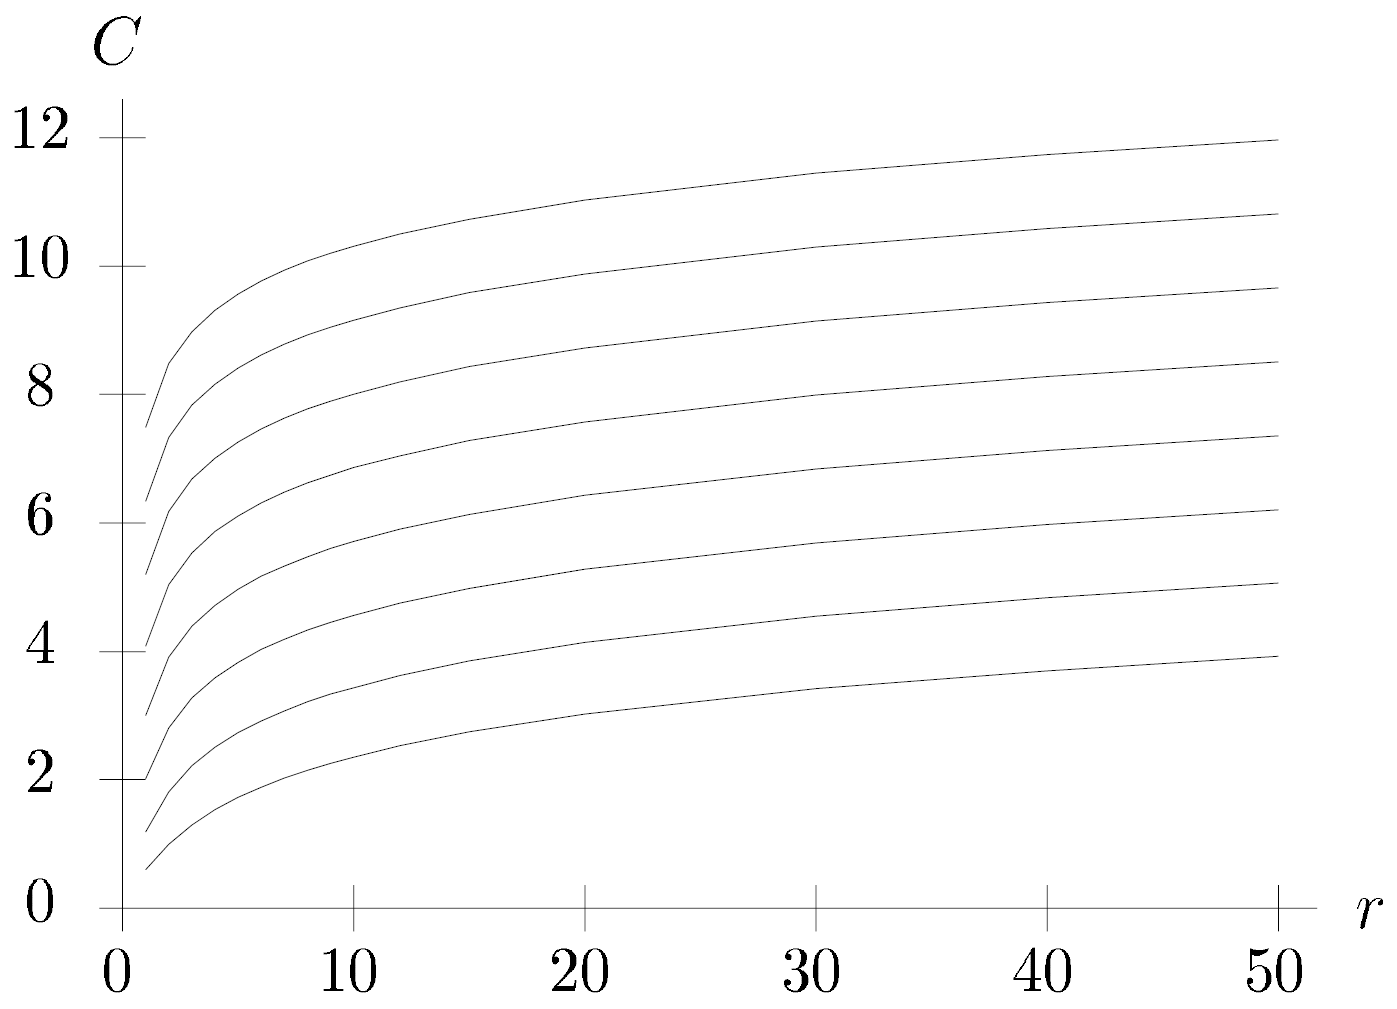
\includegraphics[width=0.6\linewidth]{img/capacity_t1}
	\caption{The value of the capacity (in \textit{nats}) for $0$dB$\leq P\leq 35$dB in $5$dB increments}
	\label{fig:capacity_t1}
\end{figure}
\end{example}

\begin{example}[$r=1$]
	In this case $m=1$ and $M=t$. Differently from before, though, the capacity is
	$$C(1,t,P) = \frac{1}{(t-1)!}
	\int_0^\infty \log(1+\frac{P}{t}\lambda)
	\lambda^{t-1} e^{-\lambda}
	\dd{\lambda}$$
	Quite differently from before, the asymptotic capacity is 
	$$C \xrightarrow{t\rightarrow\infty} \log(1+P)$$
\end{example}
Thus, just increasing the number of transmitting antennas will not help getting more capacity.

\begin{example}[$r=1$]
	\begin{figure}
		\centering
		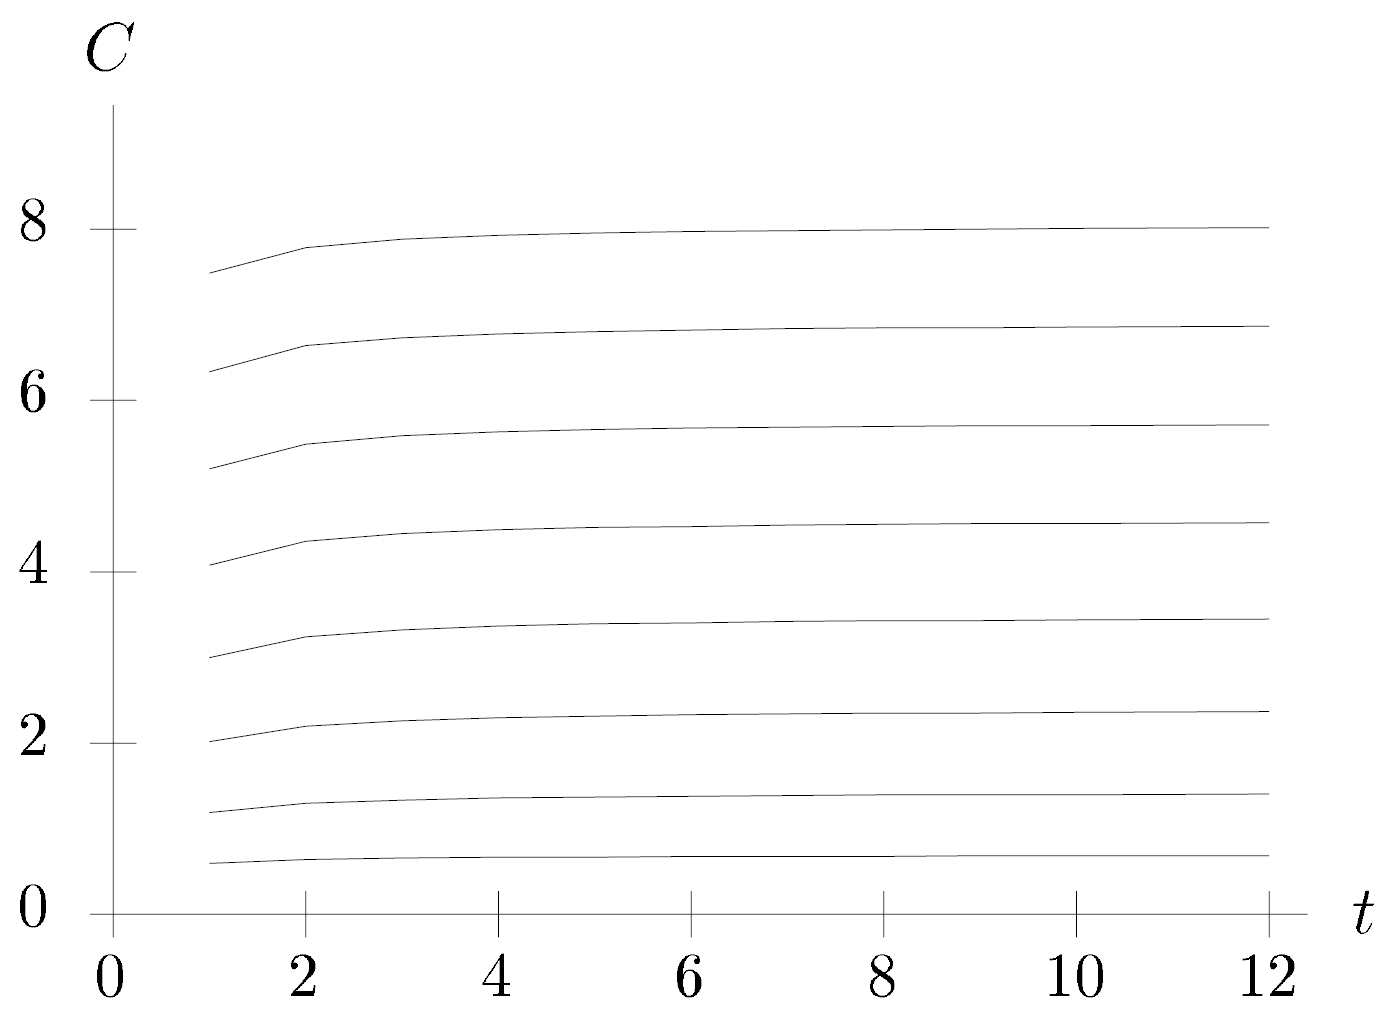
\includegraphics[width=0.6\linewidth]{img/capacity_r1}
		\caption{The value of the capacity (in \textit{nats}) for $0$dB$\leq P\leq 35$dB in $5$dB increments}
		\label{fig:capacity_r1}
	\end{figure}
\end{example}

\begin{example}[$r=t$]
	In this case $m=M=r=t$. From Eq.~\eqref{eq:capacity_ergodic}, then, we get
	$$C(m,m,P) =
	\int_0^\infty \log(1+\frac{P}{m}\lambda)
	\sum_{k=0}^{m-1} L_k(\lambda)^2 e^{-\lambda}
	\dd{\lambda}$$
	There actually exists a close form formula for this integral, which is
	\begin{equation}
	\lim_{m\rightarrow\infty} \frac{C(m,m,P)}{m} =
	\log P -1+ \frac{\sqrt{1+4P}-1}{2P} + 2\tanh[-1](\frac{1}{\sqrt{1+4P}})
	\end{equation}
	which clearly means that the capacity is a linear function of the number of transmitting/receiving antennas.
\end{example}

\begin{example}[$r=t$]
	\begin{figure}
		\centering
		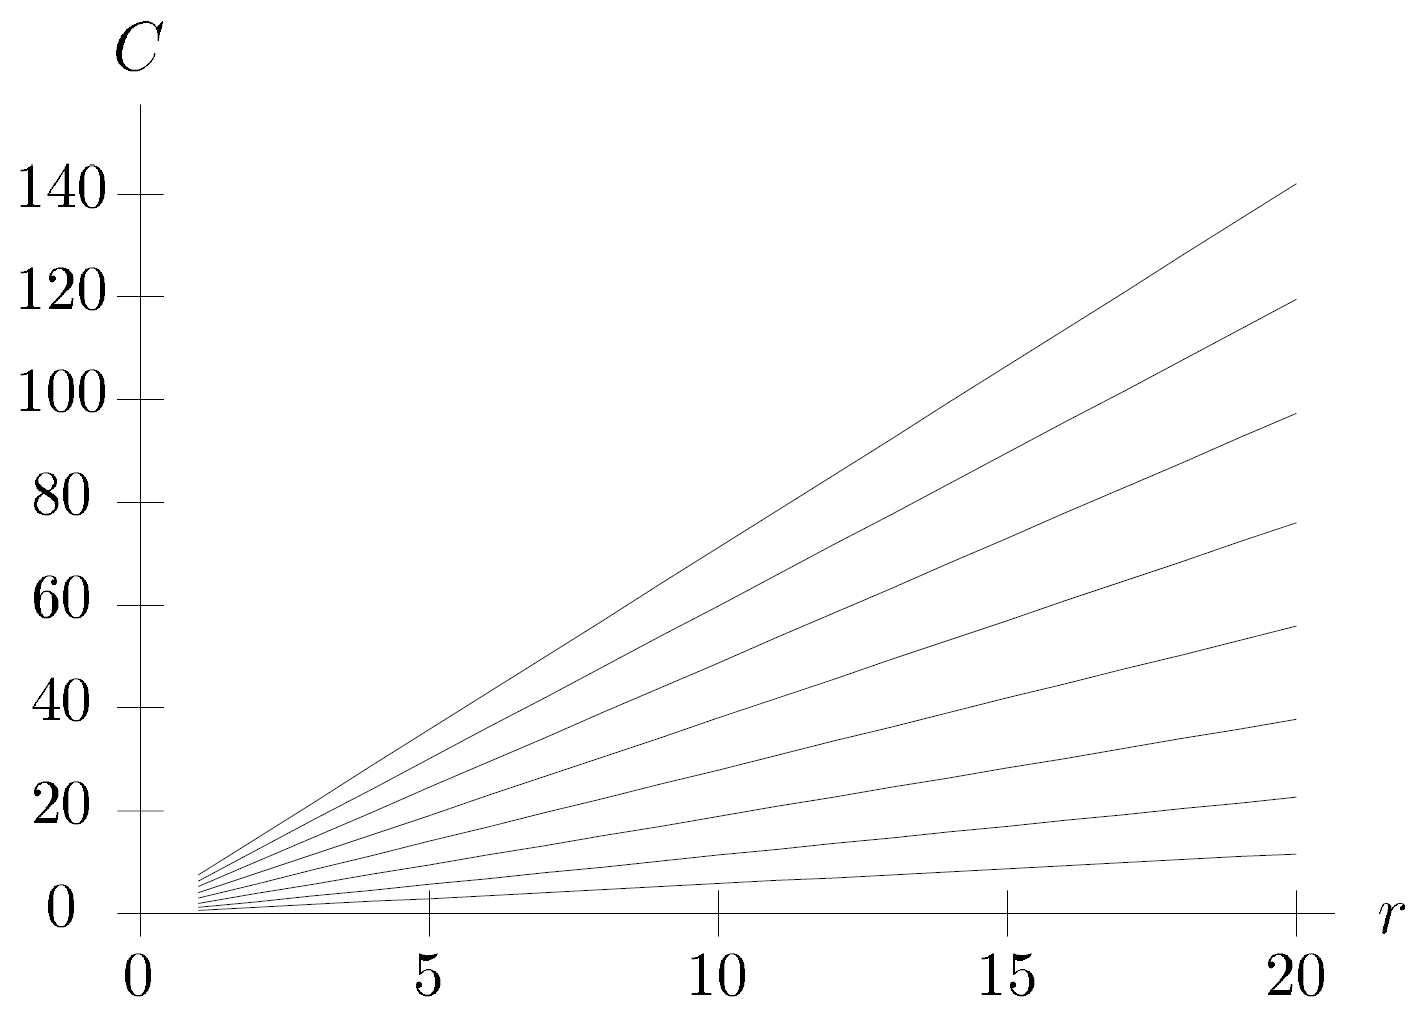
\includegraphics[width=0.7\linewidth]{img/capacity_rt}
		\caption{The value of the capacity (in \textit{nats}) for $0$dB$\leq P\leq 35$dB in $5$dB increments}
		\label{fig:capacity_rt}
	\end{figure}
\end{example}

\end{frame}